\documentclass{article}
\usepackage{graphicx}
\usepackage[ngerman]{babel}
%\usepackage{fontspec}
\usepackage{tipa}
\usepackage{natbib}
\usepackage[utf8]{inputenc}

\begin{document}

\graphicspath{ {../images/} }

%\newfontfamily{\lmln}[
%    Path=../fonts/,
%    UprightFont=Lumlun Sans Regular.ttf
%]{Lumlun Sans}
%
%\newcommand{\ortho}[1]{{\lmln\Large{\raggedright#1}\par}}

\begingroup
\centering
\vfill
\Large{Eine Vertiefungsarbeit über}\\
\Huge{KÜNSTLICHE SPRACHEN}\\
\huge{und}\\
\huge{MINIMALISTISCHE SPRACHEN}\\
\large{für die}\\
\Large{Technische Berufsschule Zürich}\\
\vspace{3cm}
\Large{von Samuel Pearce}\\
\vfill\null
\endgroup
\thispagestyle{empty}

%
% Things to mention:
% - Underlying theory -> short summary about UG
% - Language creation process
% - Experimentation process
% - Text Results
% - Review of language capacity
% - Orthography Creation -> font creation
% - Conclusion about language's capacity
% - Conclusion about minimalistic languages
% 

\begin{abstract}
    Im Laufe meiner VA habe ich versucht, die Beziehung zwischen dem Umfang einer Sprache
    (d.h. der Anzahl der allgemein gebräuchlichen Wörter und der Komplexität ihrer Grammatik)
    und ihrer Verwendbarkeit im Alltag zu entdecken und besser zu verstehen.
    Zu diesem Zweck habe ich eine Weile damit verbracht, meine eigene Sprache von Grund auf zu
    entwickeln und einige Texte in diese Sprache zu übersetzen. Dann habe ich die Texte an meine
    Freunde weitergegeben, die versucht haben, sie ins Deutsche zurück zu übersetzen.
    So konnte ich feststellen, wie schwer die Sprache zu verstehen ist.
    % TODO: Add conclusions after project.
\end{abstract}
\pagebreak

\tableofcontents
\pagebreak



\section{Einführung}



\section{Kurze Erklärung der UG Theorie}
In der Linguistik ist das Konzept der "Universellen Grammatik" auch heute noch ein heiß diskutiertes Thema.
Diese Theorie besagt, dass jeder Mensch von Geburt an die gleiche Grundstruktur für Sprache in seinem Gehirn hat.
Die moderne Form der Theorie besagt, dass es keine festen Regeln gibt, die für jede Sprache gelten,
sondern dass es Prinzipien gibt, die für jede Grammatik gelten, die aber durch Parameter angepasst werden,
was zu der fast fraktalen Komplexität aller Sprachen der Welt führt. Ein Beispiel hierfür wäre das mögliche Prinzip,
dass Satzbewegungen nur auf einen kurzen Bereich beschränkt sind, und ein Beispiel für einen Parameter ist der "Head-Parameter",
der vorschreibt, in welcher Reihenfolge Phrasen im Verhältnis zu ihrem "Kopf" gebildet werden.\cite{ChUGAI}

Der Grund, warum die Universalgrammatik eine so schwer zu knackende Nuss ist, liegt darin, dass Sprache etwas extrem Subjektives
ist und dass es - zumindest solange wir das Geheimnis des menschlichen Bewusstseins nicht gelüftet haben - unmöglich ist,
genau zu wissen, was jemand bewusst oder unbewusst zu einem bestimmten Zeitpunkt denkt. In meinem letzten Aufsatz,
in dem ich mich auf die Theorie der Universalgrammatik konzentrierte, sprach ich mich für die Verwendung konstruierter Sprachen aus,
um zu erproben, was mit der menschlichen Sprache möglich ist, und um die Tiefen unserer Sprachfähigkeiten auszuloten.

Deshalb habe ich mich entschlossen, die mir für dieses Projekt zur Verfügung stehende Zeit (und einen beträchtlichen
Teil meiner Freizeit) damit zu verbringen, die Funktionsweise von Minimalsprachen besser zu verstehen,
nachdem ich mich für das Konzept von Toki Pona, einer Sprache mit nur etwa 130 Wörtern und 7 Grammatikregeln\cite{Lang14},
begeistert hatte. Obwohl ich zugeben muss, dass dies wenig mit der Universellen Grammatik zu tun hat,
könnte es einige universelle Regeln in Bezug auf die Größe des Lexikons und den Punkt,
an dem Abstraktion zu mehrdeutig wird, aufdecken.



\section{Prozess der Spracherstellung}
Zu Beginn meiner VA und als Vorbereitung darauf begann ich, mich mit der Phonologie und Grammatik der Sprache zu beschäftigen.
Aus persönlichem Interesse verfügte ich bereits über einige Kenntnisse und Erfahrungen mit dem Prozess der Sprachentwicklung.
Ich hatte an vielen Online-Foren teilgenommen, die sich mit konstruierten Sprachen, der Konstruktion von Sprachen und der
Linguistik im Allgemeinen befassten. Der erste Schritt bestand darin, die Phonologie zu konstruieren, d. h. die Laute,
die in der Sprache verwendet werden sollten. Das war ein ziemlich einfacher Schritt, da ich mir darüber schon seit einiger
Zeit Gedanken gemacht hatte und die einfache Phonologie, die ich mir bereits ausgedacht hatte, nur noch geringfügig ändern musste.
Ich fügte auch ein System von Umlauten ein, das auf der Rundung der Vokale basiert. Dies bedeutete, dass 3 der 4 Vokale
in der Sprache von ihrer ``weichen'' Form (ungerundet für vordere Vokale und gerundet für hintere Vokale) zu ihrer ``harten'' Form
(das Gegenteil) wechseln konnten. Der Grund für den Unterschied zwischen vorderen und hinteren Vokalen war, dass vordere Vokale
in der Regel ungerundet sind, während hintere Vokale normalerweise gerundet sind.\cite{Stevens72} Durch die Abstraktion
``hart''/``weich'' klang es für die erwarteten Sprecher (Deutsch-/Englischsprecher) natürlicher.

Danach begann ich mit verschiedenen grammatikalischen Strukturen zu experimentieren und zu überlegen,
wie man sie umsetzen könnte. Obwohl dies für die Einfachheit der Sprache vielleicht keine gute Idee war,
gefiel mir die Idee, ein Groß- und Kleinschreibsystem einzuführen, um der Sprache eine freie Wortfolge zu geben.
Das habe ich mit einfachen Suffixen gemacht, die den germanischen Großbuchstabensuffixen nicht ganz unähnlich waren,
um die Mühe des Lernens auszugleichen. Danach wurde in ähnlicher Weise ein einfaches Zeitsystem mit einfachen Suffixen
für Vergangenheit, Gegenwart und Zukunft aufgebaut. Der Aspekt wurde vorerst weitgehend vernachlässigt, da er später
möglicherweise durch Hilfsadverbien ausgedrückt werden könnte.

Nachdem sich die ersten Ansätze einer Grammatik herauskristallisiert hatten, überlegte ich mir,
wie ich den erforderlichen Wortschatz reduzieren könnte, um die wenigen Wörter, die ich definieren wollte,
optimal zu nutzen. Ein Gedanke, der mir kam und absolut Sinn machte, war ein konsonantisches Wurzelsystem wie im Arabischen
oder Hebräischen, begleitet von der Idee, eine Form der Wortumkehrung einzubauen, um die Bedeutung umzukehren, d. h.,
wenn man die Wurzeln eines Wortes umkehrt, würde es sein Antonym bilden. Beides zusammen würde bedeuten, dass jemand,
der die Sprache lernt, nur eine Wurzel lernen muss und daraus bis zu 6 Bedeutungen ableiten kann.

\begin{figure}
	\centering
	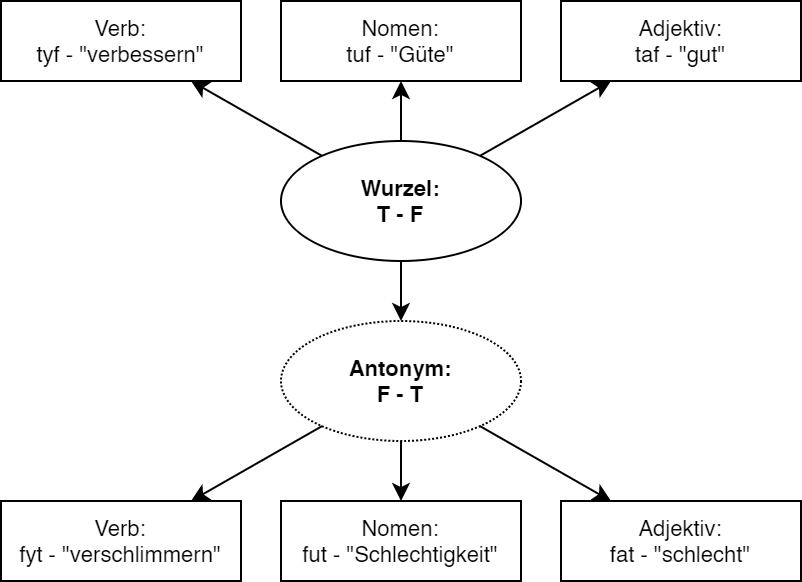
\includegraphics[scale=0.33]{root_derivations_1.png}
	\caption{Ein Diagramm aller Ableitungen der Wurzel "T-F" mit Inversion und dem bikonsonantischen Wurzelsystem.}
	\label{root_derivations_1}
\end{figure}

Danach wollte ich das System noch weiter ausbauen und schuf einige Präfixe, die unabhängig von der Wortart des Wortes
verwendet werden konnten.


\section{Prozess der Sprachprüfung}



\section{Resultate des Experiments}



\section{Kapazität der Sprache}



\section{Prozess der Erstellung der Orthografie}



\section{Schlussfolgerungen zur Nutzbarkeit meiner Sprache}



\section{Schlussfolgerungen zu minimalistischen Sprachen}


\bibliography{Bibliography}
\bibliographystyle{plain}

\end{document}